\documentclass[10pt,landscape]{article}

% Encoding
\usepackage[utf8]{inputenc}
\usepackage[T1]{fontenc}

% Document Geometry
\usepackage{multicol}
\usepackage{geometry}

% Math Environment
\usepackage{amsmath,amsfonts,amssymb}
\usepackage{gensymb}

% Images
\usepackage{float}
\usepackage{graphicx}

\title{Formulário AGO}
\author{Pedro Martins}


\geometry{top=1.2cm,left=1cm,right=1cm,bottom=1.2cm}
\pagestyle{empty}

\makeatletter
\renewcommand{\section}{\@startsection{section}{1}{0mm}%
                                {-1ex plus -.5ex minus -.2ex}%
                                {0.5ex plus .2ex}%x
                                {\normalfont\large\bfseries}}
\renewcommand{\subsection}{\@startsection{subsection}{2}{0mm}%
                                {-1explus -.5ex minus -.2ex}%
                                {0.5ex plus .2ex}%
                                {\normalfont\normalsize\bfseries}}
\makeatother

\setcounter{secnumdepth}{0}
\setlength{\parindent}{0pt}
\setlength{\parskip}{0.2cm plus4mm minus3mm}


\newcommand*\rfrac[2]{{}^{#1}\!/_{#2}}
% -----------------------------------------------------------------------

\begin{document}
\raggedright
\footnotesize

\begin{multicols}{4}
\setlength{\premulticols}{1pt}
\setlength{\postmulticols}{1pt}
\setlength{\multicolsep}{1pt}
\setlength{\columnsep}{2pt}

\begin{center}
     \Huge{{Formulário \\ $\cdot$ \\ Antenas e Guias de Onda \vspace{5mm}}} \\
\end{center}

\section{Revisões}
$Z_{IN} = \frac{Z_0^2}{Z_L}$

$\beta = \frac{2 \pi}{\lambda} $

$\Gamma_0 = \frac{Z_L - Z_0}{Z_L + Z_0}$

$VSWR = \frac{E_{max}}{E_{min}} = \frac{1 + \rho}{1 - \rho}$


\section{Parâmetros S e T}
$\begin{bmatrix} v_1^{ref} \\ v_2^{ref} \end{bmatrix} = \begin{bmatrix} s_{11} & s_{12} \\ s_{21} & s_{22} \end{bmatrix} \begin{bmatrix} v_1^{inc} \\ v_2^{inc} \end{bmatrix} $ 

$\begin{bmatrix} v_1^{inc} \\ v_1^{ref} \end{bmatrix} = \begin{bmatrix} t_{11} & t_{12} \\ t_{21} & t_{22} \end{bmatrix} \begin{bmatrix} v_2^{ref} \\ v_2^{inc} \end{bmatrix} $ 

$\begin{bmatrix} t_{11} & t_{12} \\ t_{21} & t_{22} \end{bmatrix} = \begin{bmatrix} \frac{1}{S_{21}} & -\frac{S_{22}}{S_{21}} \\ \frac{S_{11}}{S_{21}} & S_{12} - \frac{S_{11}S_{22}}{S_{21}}\end{bmatrix}$ 

$\begin{bmatrix} S_{11} & S_{12} \\ S_{21} & S_{22} \end{bmatrix} = \begin{bmatrix} \frac{T_{21}}{T_{11}} & T_{22} - \frac{T_{21}T_ {12}}{T_{11}} \\ \frac{1}{T_{11}} & -\frac{T_{12}}{T_{11}}\end{bmatrix}$ 

\section{Amplificadores}
$\rho_{IN} = S_{11} + \frac{S_{12}S_{21}\rho_L}{1 - S_{22}\rho_L}$

$\rho_{OUT} = S_{22} + \frac{S_{12}S_{21}\rho_S}{1 - S_{11}\rho_S}$

$G_T = \frac{P_L}{P_{AVS}} = \frac{1 - |\Gamma_s|^2}{|1 - \Gamma_{IN}\Gamma_s|^2} |S_{21}|^2 \frac{1 - |\Gamma_L|^2}{|1 - S_{22}\Gamma_L|^2}$ 

$G_A = \frac{P_{AVL}}{P_{AVS}} = \frac{1 - |\Gamma_s|^2}{|1 - S_{11}\Gamma_s|^2} |S_{21}|^2 \frac{1}{1 - |\Gamma_{OUT}|^2}$

$G_P = \frac{P_{L}}{P_{IN}} = \frac{1}{1 - |\Gamma_{IN}|^2} |S_{21}|^2 \frac{1 - |\Gamma_L|^2}{|1 - S_{22}\Gamma_L|^2}$

$G_{TU} = \frac{1 - |\Gamma_s|^2}{|1 - S_{11}\Gamma_s|^2} |S_{21}|^2 \frac{1 - |\Gamma_L|^2}{|1 - S_{22}\Gamma_L|^2}$

$G_{TU, max} = \frac{1}{|1 - S_{11}|^2} |S_{21}|^2 \frac{1}{|1 - S_{22}|^2}$

$G_T = \frac{P_L}{P_{AVS}} = \frac{P_{AVL}}{P_{AVS}} \frac{P_{L}}{P_{AVL}} = G_A L_L$

$G_T = \frac{P_L}{P_{AVS}} = \frac{P_{IN}}{P_{AVS}} \frac{P_{L}}{P_{IN}} = L_S G_P$



\subsection{Estabilidade}
$|\Gamma_S| < 1  \wedge |\Gamma_L| < 1 \wedge |\Gamma_{IN}| < 1 \wedge |\Gamma_{OUT}| < 1$

\section{Filters}
$L = \frac{g_k Z_0}{2 \pi f_c}$

$C = \frac{g_k}{2 \pi Z_0 f_c}$

\subsection{Transformada de Richards}
$\omega_c = tan(\beta l) $

$Z = j g_k \omega_c \Rightarrow Z = j Z_0 \tan(\beta l) \hfill \wedge  Z_0 = g_k$ 

$Y = j g_k \omega_c \Rightarrow Y = \frac{j \tan(\beta l)}{Z_0}  \hfill \wedge  Z_0 = \frac{1}{g_k}$ 


\subsection{Maximum Flat (3dB)}
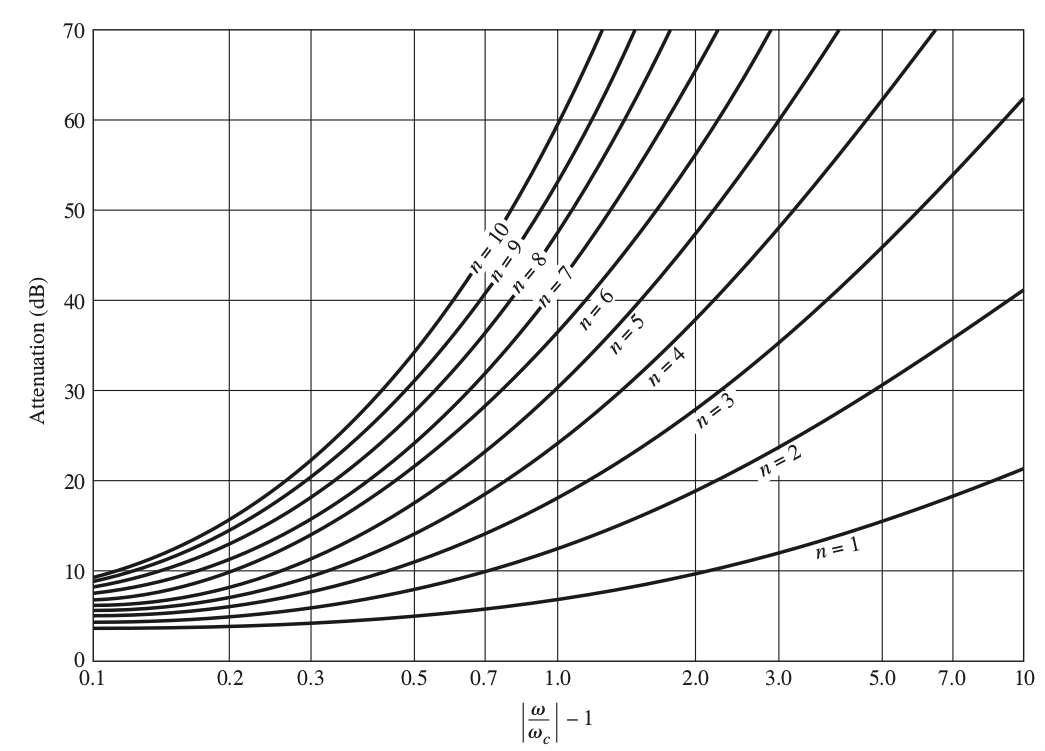
\includegraphics[width=0.2\textwidth]{flat.png}
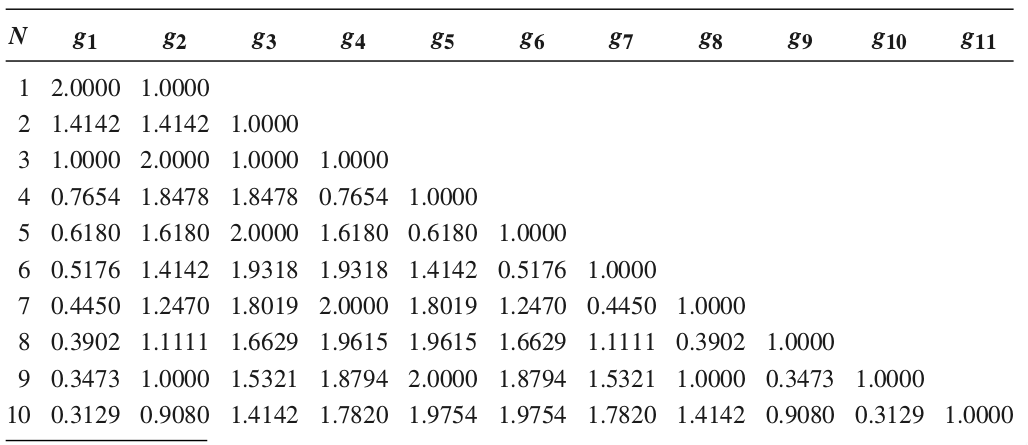
\includegraphics[width=0.3\textwidth, angle=90]{maximum_flat_table_3dB.png}

\subsection{Equal Ripple (3dB)}
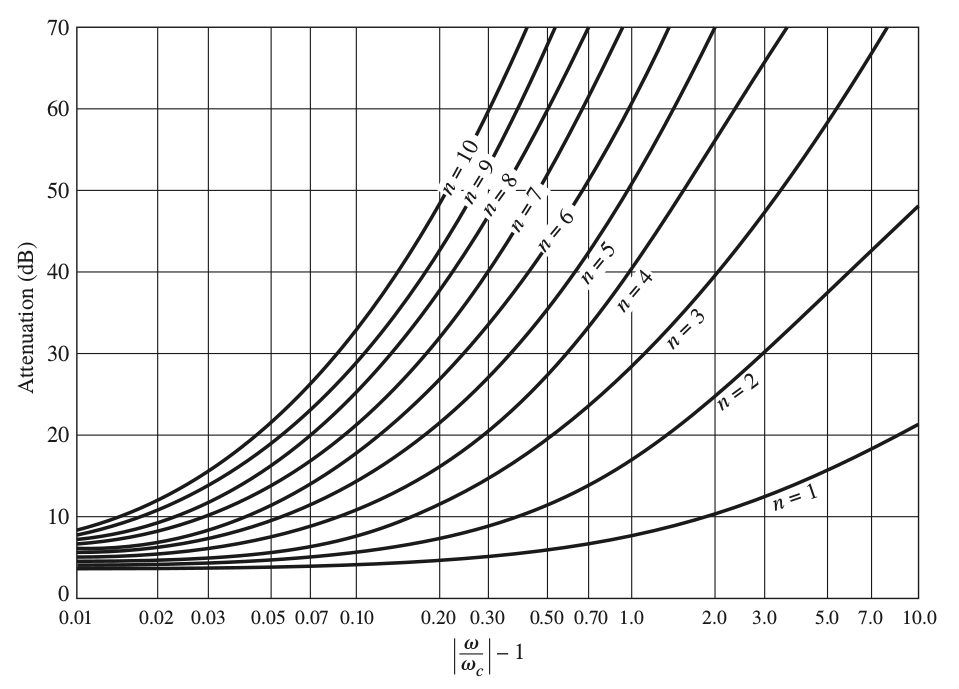
\includegraphics[width=0.2\textwidth]{equal_ripple_3dB.png}
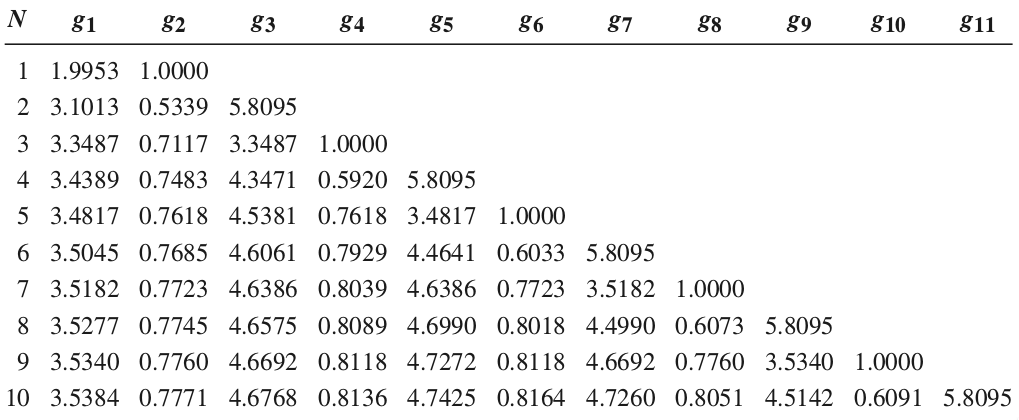
\includegraphics[width=0.3\textwidth, angle=90]{equal_ripple_table_3dB.png}

\subsection{Koroda}
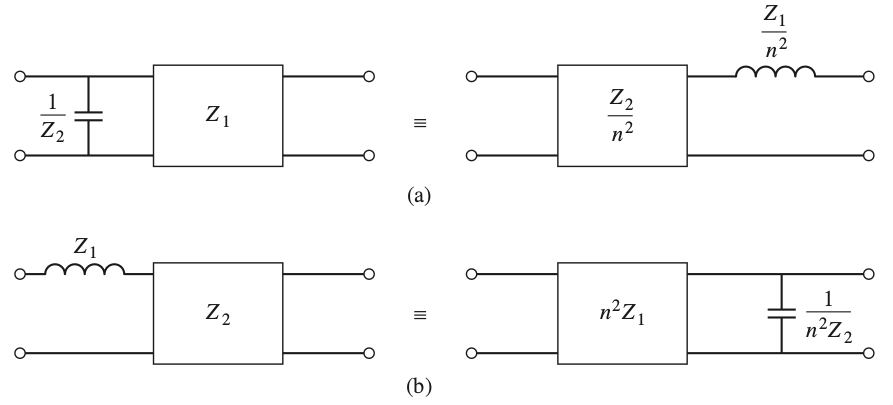
\includegraphics[width=0.2\textwidth]{Kuroda.png}
$n^2 = 1 + \frac{Z_2}{Z_1}$

\subsection{Frequency Transformations}
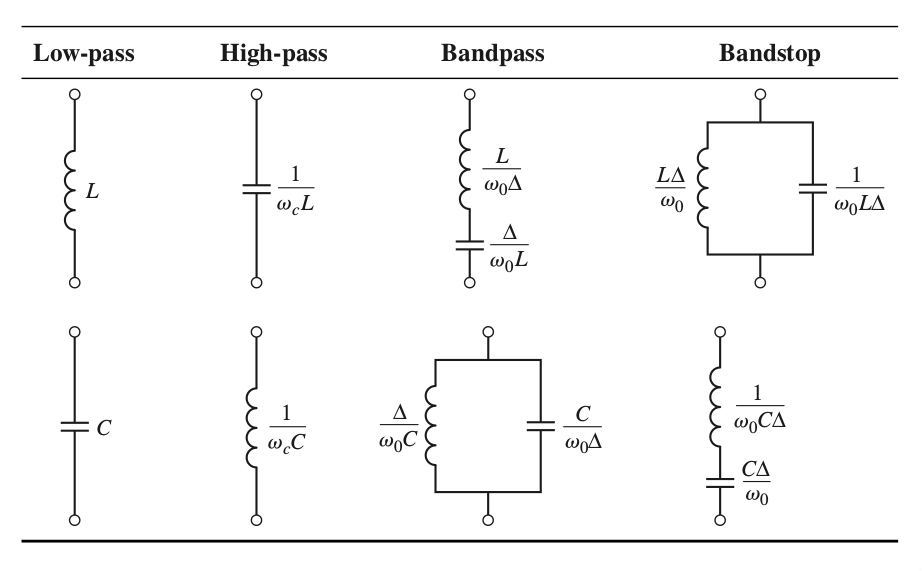
\includegraphics[width=0.2\textwidth]{filter_transform.png}
$\Delta = \frac{\omega_2 - \omega_1}{\omega_0}$

\subsection{Stepped Impedance}
Bobine $\rightarrow \beta l = \frac{L Z_0}{Z_{high}}$ 

Condensador $\rightarrow \beta l = \frac{C Z_{low}}{Z_{0}}$ 

\section{Guias de Onda}
\begin{tabular}{lll}
$E_z =    0$ & $H_z =    0$ & Modos TEM \\
$E_z =    0$ & $H_z \neq 0$ & Modos TE ou H \\
$E_z \neq 0$ & $H_z =    0$ & Modos TM ou E \\
$E_z \neq 0$ & $H_z \neq 0$ & Modos Híbridos \\
\end{tabular}

\vspace{2mm}

\begin{tabular}{l|l}
$\epsilon_0$  & $8.854187817 \times 10^{-12} F\cdot m^{-1}$ \\ 
$\mu_0$  & $4\pi \times 10^{-7} H\cdot m^{-1}$ \\
\end{tabular}

\vspace{2mm}

$k_c^2 = k^2 - \beta^2$ 

$\eta = 120 \pi \rightarrow$ Impedância Característica do ar

\subsection{Retangulares}
O modo TM não se propaga se $n = 0$ ou $m = 0$ \\
$\lambda_0 \rightarrow$ Comprimento de onda em meio livre \\
$\lambda_{0c} \rightarrow$ Comprimento de onda de corte no meio \\

$k = \omega \sqrt{\mu\epsilon} = \frac{2 \pi}{\lambda}$ \\
$f_{c_{mn}} = \frac{v}{2} \sqrt{\left(\frac{n}{y_1}\right)^2 + \left(\frac{m}{z_1}\right)^2}$ \\
$\lambda_{c_{mn}} = \frac{2}{\sqrt{\left(\frac{n}{y_1}\right)^2 + \left(\frac{m}{z_1}\right)^2}}$ \\

$\beta = \sqrt{k^2 - k_c^2} = \sqrt{k^2 - \left(\frac{n}{y_1}\right)^2 - \left(\frac{m}{z_1}\right)^2}$ 

$k_c^2 = \left(\frac{n}{y_1}\right)^2 - \left(\frac{m}{z_1}\right)^2$\\

$\gamma = \alpha_d + j\beta = \sqrt{k_c^2 - k^2}$ \\

$\gamma = \sqrt{\left(\frac{n}{y_1}\right)^2 - \left(\frac{m}{z_1}\right)^2 - \omega^2\mu\epsilon} = \sqrt{k_c^2 - \beta_0^2}$ 

$v_p = \frac{\omega}{\beta} = \frac{v_0}{\sqrt{1 - \left(\frac{n\lambda_0}{2y_1}\right)^2 - \left(\frac{m\lambda_0}{2z_1}\right)^2 }} = \frac{v_0}{\sqrt{1 - \left(\frac{\lambda_0}{\lambda_{0c}}\right)^2}}$ 

$Z_{TE} = \frac{k\eta}{\beta}$ 
e se $f > f_c, Z_{TE} = \frac{Z_d}{\sqrt{1 - \left(\frac{\lambda_0}{\lambda_{0c}}\right)^2}} $

$v = \frac{c}{\sqrt{\epsilon_r}}$

$\lambda = \frac{\lambda_0}{\sqrt{\epsilon_r}}$

\subsection{Cilíndrico}
$n \rightarrow$ ordem da função de Bessel \\
$k \rightarrow$ raiz da ordem n da função de Bessel \\
$k' \rightarrow$ raiz da ordem n da derivada da função de Bessel \\
$a  \rightarrow$ raio do guia de onda \\
$p_{nm} \rightarrow$ raiz de ordem m da função de Bessel de ordem n \\
$p'_{nm} \rightarrow$ raiz de ordem m da derivada da função de Bessel de ordem n \\

Os modos TE e TM obrigam a $m \neq 0$

\subsubsection{Modo $TE_{nm}$}
$k_{c_{nm}} = \frac{p'_{nm}}{a}$ \\

$\beta_{nm} = \sqrt{k^2 - k^c} = \sqrt{k^2 - \left(\frac{p'_{nm}}{r}\right)^2}$ \\

$f_{c_{nm}} = \frac{k_c}{2\pi\sqrt{\mu\epsilon}} = \frac{p'_{nm}}{2\pi a \sqrt{\mu\epsilon}}$

$f_c = \frac{v}{2\pi} \frac{k'nm}{a}$ \\

$\lambda_c = \frac{2\pi a}{k' nm}$ \\

$Z_{TE} = \frac{\eta k}{\beta}$ \\

\resizebox{0.25\textwidth}{!}{%
\begin{tabular}{l|llllll}
k & $J_0$'(x) & $J_1$'(x) & $J_2$'(x) & $J_3$'(x) & $J_4$'(x) & $J_5$'(x) \\  \hline
1 & 3.8317    & 1.8412    & 3.0542    & 4.2012    & 5.3175    & 6.4156    \\
2 & 7.0156    & 5.3314    & 6.7061    & 8.0152    & 9.2824    & 10.5199   \\
3 & 10.1735   & 8.5363    & 9.9695    & 11.3459   & 12.6819   & 13.9872   \\
4 & 13.3237   & 11.7060   & 13.1704   & 14.5858   & 15.9641   & 17.3128   \\
5 & 16.4706   & 14.8636   & 16.3475   & 17.7887   & 19.1960   & 20.5755   \\                
\end{tabular}
}



\subsubsection{Modo TM}
$k_{cm} = \frac{p_{nm}}{a}$ \\

$\beta_{nm} = \sqrt{k^2 - k^c} = \sqrt{k^2 - \left(\frac{p'_{nm}}{r}\right)^2}$ \\

$f_{c_{nm}} = \frac{k_c}{2\pi\sqrt{\mu\epsilon}} = \frac{p_{nm}}{2\pi a \sqrt{\mu\epsilon}}$ \\

$f_c = \frac{v}{2\pi} \frac{knm}{a}$ \\

$\lambda_c = \frac{2\pi a}{k nm}$ \\

$Z_{TM} = \frac{\eta \beta}{k}$ \\

\resizebox{0.25\textwidth}{!}{%
\begin{tabular}{l|llllll}
k & $J_0$(x)  & $J_1$(x)  & $J_2$(x)  & $J_3$(x)  & $J_4$(x)  & $J_5$(x)  \\ \hline
1 & 2.4048   & 3.8317     & 5.1356    & 6.3802    & 7.5883    & 8.7715    \\
2 & 5.5201   & 7.0156     & 8.4172    & 9.7610    & 11.0647   & 12.3386   \\
3 & 8.6537   & 10.1735    & 11.6198   & 13.0152   & 14.3725   & 15.7002   \\
4 & 11.7915  & 13.3237    & 14.7960   & 16.2235   & 17.6160   & 18.9801   \\
5 & 14.9309  & 16.4706    & 17.9598   & 19.4094   & 20.8269   & 22.2178   \\
\end{tabular}
}

\subsection{Perdas}
Dielétrico $\rightarrow \alpha_d = \omega\epsilon \tan(\delta)$ \\
$\alpha_{d_{mn}} = \frac{\omega \tan(\delta)}{2c\sqrt{1 - \left(\frac{f_{c_{mn}}}{f}\right)^2}} = \frac{\omega\sqrt{\mu\epsilon} \tan (\delta)}{2 \beta} = \frac{k^2 \tan(\delta)}{2\beta}$ \\

Não há propagação ($f < f_c$): \\

$\alpha = \frac{2\pi}{\lambda} \sqrt{\left(\frac{\lambda}{\lambda_c}\right)^2 - 1} $

Há propagação ($f > f_c$): \\

$\alpha_d = \frac{\pi \tan(\delta)}{\lambda \sqrt{ 1 - \frac{\lambda}{\lambda_c}}} $ \\
$\alpha_c = \frac{Re[Z_c]}{Z_d y_1} \frac{1 + 2 \frac{y_1}{x_1} \left(\frac{\lambda}{\lambda_c}\right)^2}{\sqrt{1 - \left(\frac{\lambda}{\lambda_c}\right)^2}}$\\

$P_{max} = \frac{E^2 y_1 z_1}{4 Z_{TE}}$\\

$R_S = \frac{1}{\sigma \delta} = \sqrt{\frac{\omega \mu}{2 \sigma}} \rightarrow$ Efeito de Skin \\

\subsection{Propagação ($f > f_c$)}
$\gamma = \pm \sqrt{\left(\frac{p'_{nm}}{a}\right)^2 - \omega^2\mu\epsilon}$ \\
$f_c = \frac{1}{2\pi \sqrt{\mu\epsilon}} \frac{p'_{nm}}{a}$ \\
$\lambda_{0c} = \frac{2\pi a}{p'_{nm}}$ \\
$\beta = \sqrt{\omega^2 \mu\epsilon - \left(\frac{p'_{nm}}{a}\right)^2}$ \\
$\lambda_{g} = \frac{\lambda_0}{\sqrt{1 - \left(\rfrac{\lambda_0}{\lambda_{0c}}\right)^2}}$ \\
$v_p = \frac{\omega}{\beta} = \frac{v_0}{\sqrt{1 - \left(\rfrac{\lambda_0}{\lambda_{0c}}\right)^2}}, \qquad v_0 = \rfrac{1}{\sqrt{\mu\epsilon}}$

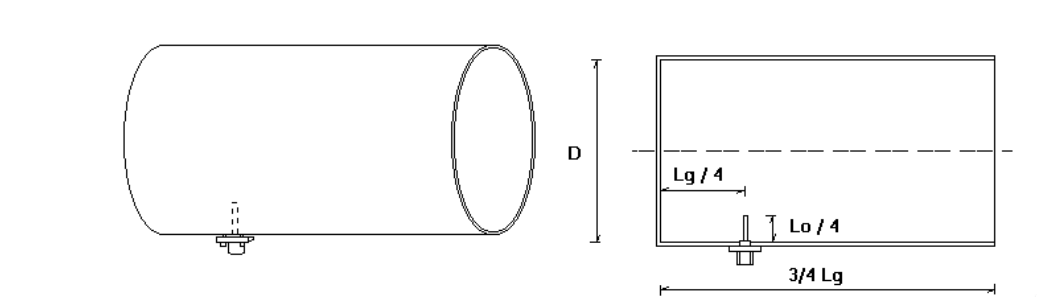
\includegraphics[width=0.24\textwidth]{propagation.png}

\section{Fibras}
$\sin (\theta_2) = \left(\frac{\mu_1}{\mu_2}\right) \sin(\theta_2)$ \\

$\theta_1 = \theta_c \Rightarrow \theta_2 = 90 \degree$ \\

$\sin(\theta_c) =\frac{n_2}{n_1}$ \\

$\sin [\theta_{i_{max}}] = \frac{\sqrt{n_1^2 - n_2^2}}{n_0}$ \\

Fractional Difference $\rightarrow \Delta = \frac{n_1 - n_2}{n_1}$ \\

Guide light effective $\Rightarrow \Delta << 1$ \\

$NA = n_1 \sqrt{2\Delta}$ \\

$\theta$ close to $\theta_{critical} \Rightarrow$ Higher order modes \\

$\theta$ larger than $\theta_{critical} \Rightarrow$ Lower order modes \\

$v = \frac{2 \pi d}{\lambda} \sqrt{\mu_1^2 - \mu_2^2} = \frac{2 \pi d}{\lambda} NA$ \\

$M = \frac{V^2}{2}$ \\

Velocidade de Fase $\rightarrow v_f = \frac{\omega}{k} = \frac{c}{n}$ \\

Velocidade de Grupo $\rightarrow v_g = \frac{d\omega}{dk} = \frac{c}{m}$ \\

$m = n - \lambda_0\frac{dn}{d\lambda_0}$ \\

\section{Antenas}
Diretividade $\rightarrow D(\theta, \Phi) = \frac{U(\theta, \Phi)}{U_0}$ \\

Na direção de máximo $\rightarrow D(\theta, \Phi) = 4\pi \frac{U_{max}}{P_{rad}}$ \\

$G(\theta, \Phi) = \frac{U(\theta, \Phi)}{U_0} = 4\pi \frac{U_{max}}{P_{in}}$ \\

Densidade de uma antena isotrópica sem perdas:

$U_0 = \frac{P_{rad}}{4\pi} = \frac{P_{in}}{4\pi}$ \\

$U(\theta, \Phi) = R^2 S_{rad} = R^2 \frac{1}{2} \frac{|E_\theta|^2}{\eta}$ \\

$G(\theta, \Phi) = e_t D(\theta, \Phi) $ \\

$\rho = \frac{P_{rad}}{P_{IN}}$ \\

\subsection{Potência}
$P_{in} = P_{rad} + P_{D}$ \\

$P_D = P_{ref} + P_c + P_d$ \\

$P_{ref} \rightarrow$ Potência refletida por desaptação \\
$P_{c} \rightarrow$ Potência dissipada nas paredes condutoras da antena \\
$P_{d} \rightarrow$ Potência dissipada no dielétrico \\

\subsection{Eficiência}
eficiência $\rightarrow e_t = \frac{P_{rad}}{P_{in}} = e_r e_c e_d$ \\

Eficiência de Radiação $\rightarrow e_{cd} = e_c e_d$ \\

$S_{rad} = \frac{1}{2} (E \times H^*)$ \\

$e_r = \frac{P_{tran}}{P_{in}} = (1 - |\rho|^2) $ \\

\subsection{Impedância}
$Z_A = R_A + jX_A \Rightarrow R_A = R_r + R_p$ \\

Efeito de Skin $\rightarrow \delta = \sqrt{\frac{2}{\omega\mu\sigma}}$ \\

\subsection{Effective Area}
$A_e = \frac{P_T}{S_i} = $\\

$S_{isotropica} = \frac{P_{rad1}}{4\pi r^2}$ \\

$S_{1} = D_1 \frac{P_{rad1}}{4\pi r^2}$ \\

$S_i \rightarrow$ Densidade de Potência \\

$A_e = \frac{\lambda^2}{4 \pi} G$

\subsection{Transmissão}
$P_{rad} = e_{t1} P_{in}$ \\
$G_1 = e_{t1} D_1$ \\

$P_T = A_{e2} S_1 =  A_{e2} G_1 \frac{P_{in}}{4\pi r^2}$\\

$|E_\theta| = \frac{\eta I \Delta Z}{2\pi R \lambda} \sin(\theta)$

\subsection{Fórmula de Friis}
$P_T = A_{e2} \frac{P_{in}}{4 \pi r^2} G_1 = P_{in} \left(\frac{\lambda}{4 \pi r}\right)^2 G_t G_r$ \\

$\left(\frac{\lambda}{4 \pi r}\right)^2 \rightarrow$ Perdas em espaço livre \\

\subsection{Radar}
$P_{ref} = S_i \sigma$ \\

$P = A_e S_A = P_t \sigma G^2 \frac{1}{4\pi} \left(\frac{\lambda}{4\pi r^2}\right)^2$ \\

\section{Antenas Filiformes}

$H_\Phi = j \frac{\beta I \Delta z}{4 \pi r} e^{-j\beta r} \sin(\theta)$ \\

$E_\theta = j \eta \frac{\beta I \Delta z}{4 \pi r} e^{-j\beta r} \sin(\theta)$ \\

\subsection{Dipolo}
$P = P_{rad} + jQ = \eta \frac{\pi}{3} \left(\frac{I \Delta z}{\lambda}\right)^2 \left[1 - j \frac{1}{(\beta r)^3}\right]$ \\

$\eta = \sqrt{\frac{\mu}{\epsilon}}$ \\

Em campo distante ($f >> \lambda$), Q é desprezável face a $P_{rad}$ \\

Resistência de Radiação $\rightarrow R_r = \eta \frac{2\pi}{3}\left(\frac{\Delta z}{\lambda}\right)^2$ \\

$U(\theta, \Phi) = r^2 S = r^2 \frac{1}{2}\left(\frac{|E|^2}{\eta}\right)$\\

$U(\theta) = r^2 S_{rad} = \frac{\eta}{2}\left(\frac{\beta I \Delta z}{4 \pi}\right)^2 \sin^2(\theta)$ \\

$D(\theta, \Phi) = 4 \pi \frac{U(\theta, \Phi)}{P_{rad}}$ \\

$A_e = \frac{\lambda^2}{4 \pi} D$ \\

Num dipolo curto, $U_{max}$, $P_{rad}$ e $R_r$ passa para $\rfrac{1}{4}$.\\

$U(\theta) = R^2 S_{rad}(\theta, \Phi, R)$ \\

$S_{rad} = \frac{\eta |I_0|^2}{8 \pi^2 R^2} \left[\frac{\cos\left(\frac{pi}{2}cos(\theta)\right)}{\sin(\theta)}\right]^2$ \\

$U_n(\theta, \Phi) = \left(\frac{\cos\left(\frac{pi}{2}cos(\theta)\right)}{\sin(\theta)}\right)^2$

\subsection{Monopolo}
$E_2^{mono} = E_2^{di} \Rightarrow S_\theta^{mono} = S_\theta^{di} \Rightarrow U_\theta^{mono} = U_\theta^{di}, se \theta \leq \frac{\pi}{2}$\\

$P_{rad}^{mono} = \frac{1}{2} P_{rad}^{di}$ \\

$D^{mono} = 2 D^{di}$ \\

$|E_g| = \frac{\eta I_0}{2 \pi R}$

\section{Antenas Microstrip}
$W = \frac{1}{2f_r \cdot \sqrt{\epsilon_0 \mu_0}} \sqrt{\frac{2}{\epsilon_r + 1}}$ \\
$\epsilon_{reff} = \frac{\epsilon_r + 1}{2} + \frac{\epsilon_r - 1}{2\cdot \sqrt{1 + \frac{12d}{W}}}$ \\
$\Delta L = 0.412d \cdot \left(\epsilon_{reff} + 0.3\right) \frac{\frac{W}{d} + 0.264}{\left(\epsilon_{reff} -0.258\right)\left(\frac{W}{d} + 0.8\right)} $\\
$L = \frac{1}{2 f_r \sqrt{\epsilon_{reff}} \cdot \sqrt{\epsilon_0 \mu_0}} - 2\Delta L$ \\
$Z_a = 90 \frac{\epsilon_r^2}{\epsilon_r - 1} \left(\frac{L}{W}\right)^2$ \\


\subsection{Agregados de Antenas}
$\phi = \beta d \cos(\theta) + \alpha$ \\

$E_{\theta T} = j\eta \frac{I_0e^{-j\beta R}}{2\pi R} \left[\frac{\cos\left(\frac{pi}{2}cos(\theta)\right)}{\sin(\theta)}\right]\left[2cos\left(\frac{\beta d \cos(\theta) + \alpha}{2}\right)\right]$

$FA = \frac{\sin(N\frac{\phi}{2})}{\sin(\frac{\phi}{2})}$


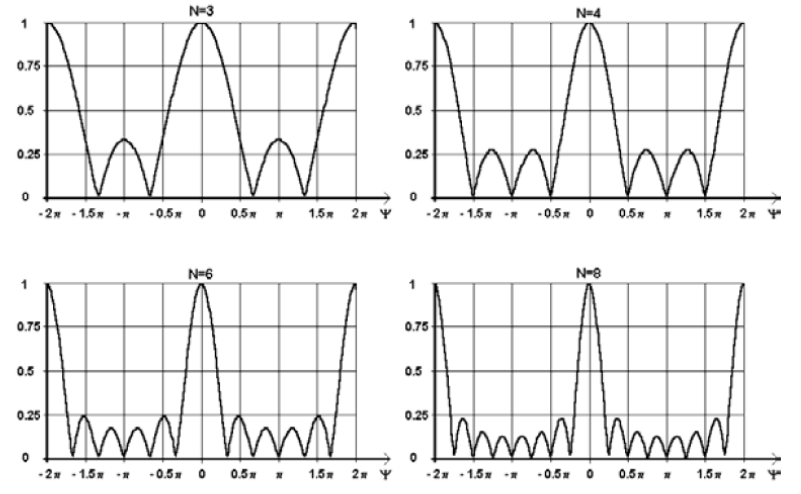
\includegraphics[width=0.25\textwidth]{radiation_diagram.png}



{\scriptsize \raggedleft  Pedro Martins (martinspedro@ua.pt)}

\end{multicols}
\end{document}
